\documentclass[twoside]{book}

% Packages required by doxygen
\usepackage{fixltx2e}
\usepackage{calc}
\usepackage{doxygen}
\usepackage[export]{adjustbox} % also loads graphicx
\usepackage{graphicx}
\usepackage[utf8]{inputenc}
\usepackage{makeidx}
\usepackage{multicol}
\usepackage{multirow}
\PassOptionsToPackage{warn}{textcomp}
\usepackage{textcomp}
\usepackage[nointegrals]{wasysym}
\usepackage[table]{xcolor}

% Font selection
\usepackage[T1]{fontenc}
\usepackage[scaled=.90]{helvet}
\usepackage{courier}
\usepackage{amssymb}
\usepackage{sectsty}
\renewcommand{\familydefault}{\sfdefault}
\allsectionsfont{%
  \fontseries{bc}\selectfont%
  \color{darkgray}%
}
\renewcommand{\DoxyLabelFont}{%
  \fontseries{bc}\selectfont%
  \color{darkgray}%
}
\newcommand{\+}{\discretionary{\mbox{\scriptsize$\hookleftarrow$}}{}{}}

% Page & text layout
\usepackage{geometry}
\geometry{%
  a4paper,%
  top=2.5cm,%
  bottom=2.5cm,%
  left=2.5cm,%
  right=2.5cm%
}
\tolerance=750
\hfuzz=15pt
\hbadness=750
\setlength{\emergencystretch}{15pt}
\setlength{\parindent}{0cm}
\setlength{\parskip}{3ex plus 2ex minus 2ex}
\makeatletter
\renewcommand{\paragraph}{%
  \@startsection{paragraph}{4}{0ex}{-1.0ex}{1.0ex}{%
    \normalfont\normalsize\bfseries\SS@parafont%
  }%
}
\renewcommand{\subparagraph}{%
  \@startsection{subparagraph}{5}{0ex}{-1.0ex}{1.0ex}{%
    \normalfont\normalsize\bfseries\SS@subparafont%
  }%
}
\makeatother

% Headers & footers
\usepackage{fancyhdr}
\pagestyle{fancyplain}
\fancyhead[LE]{\fancyplain{}{\bfseries\thepage}}
\fancyhead[CE]{\fancyplain{}{}}
\fancyhead[RE]{\fancyplain{}{\bfseries\leftmark}}
\fancyhead[LO]{\fancyplain{}{\bfseries\rightmark}}
\fancyhead[CO]{\fancyplain{}{}}
\fancyhead[RO]{\fancyplain{}{\bfseries\thepage}}
\fancyfoot[LE]{\fancyplain{}{}}
\fancyfoot[CE]{\fancyplain{}{}}
\fancyfoot[RE]{\fancyplain{}{\bfseries\scriptsize Generated by Doxygen }}
\fancyfoot[LO]{\fancyplain{}{\bfseries\scriptsize Generated by Doxygen }}
\fancyfoot[CO]{\fancyplain{}{}}
\fancyfoot[RO]{\fancyplain{}{}}
\renewcommand{\footrulewidth}{0.4pt}
\renewcommand{\chaptermark}[1]{%
  \markboth{#1}{}%
}
\renewcommand{\sectionmark}[1]{%
  \markright{\thesection\ #1}%
}

% Indices & bibliography
\usepackage{natbib}
\usepackage[titles]{tocloft}
\setcounter{tocdepth}{3}
\setcounter{secnumdepth}{5}
\makeindex

% Hyperlinks (required, but should be loaded last)
\usepackage{ifpdf}
\ifpdf
  \usepackage[pdftex,pagebackref=true]{hyperref}
\else
  \usepackage[ps2pdf,pagebackref=true]{hyperref}
\fi
\hypersetup{%
  colorlinks=true,%
  linkcolor=blue,%
  citecolor=blue,%
  unicode%
}

% Custom commands
\newcommand{\clearemptydoublepage}{%
  \newpage{\pagestyle{empty}\cleardoublepage}%
}

\usepackage{caption}
\captionsetup{labelsep=space,justification=centering,font={bf},singlelinecheck=off,skip=4pt,position=top}

%===== C O N T E N T S =====

\begin{document}

% Titlepage & ToC
\hypersetup{pageanchor=false,
             bookmarksnumbered=true,
             pdfencoding=unicode
            }
\pagenumbering{roman}
\begin{titlepage}
\vspace*{7cm}
\begin{center}%
{\Large My Project }\\
\vspace*{1cm}
{\large Generated by Doxygen 1.8.11}\\
\end{center}
\end{titlepage}
\clearemptydoublepage
\tableofcontents
\clearemptydoublepage
\pagenumbering{arabic}
\hypersetup{pageanchor=true}

%--- Begin generated contents ---
\chapter{Class Index}
\section{Class List}
Here are the classes, structs, unions and interfaces with brief descriptions\+:\begin{DoxyCompactList}
\item\contentsline{section}{\hyperlink{structnode}{node} }{\pageref{structnode}}{}
\item\contentsline{section}{\hyperlink{structnode1}{node1} }{\pageref{structnode1}}{}
\item\contentsline{section}{\hyperlink{structnode__info}{node\+\_\+info} }{\pageref{structnode__info}}{}
\end{DoxyCompactList}

\chapter{File Index}
\section{File List}
Here is a list of all files with brief descriptions\+:\begin{DoxyCompactList}
\item\contentsline{section}{\hyperlink{Lab1_8c}{Lab1.\+c} }{\pageref{Lab1_8c}}{}
\end{DoxyCompactList}

\chapter{Class Documentation}
\hypertarget{classRandomizedBinarySearchTree}{}\section{Randomized\+Binary\+Search\+Tree Class Reference}
\label{classRandomizedBinarySearchTree}\index{Randomized\+Binary\+Search\+Tree@{Randomized\+Binary\+Search\+Tree}}


Collaboration diagram for Randomized\+Binary\+Search\+Tree\+:
\nopagebreak
\begin{figure}[H]
\begin{center}
\leavevmode
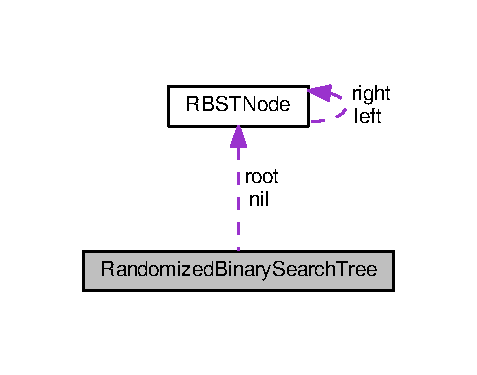
\includegraphics[width=229pt]{classRandomizedBinarySearchTree__coll__graph}
\end{center}
\end{figure}
\subsection*{Public Member Functions}
\begin{DoxyCompactItemize}
\item 
\hyperlink{classRandomizedBinarySearchTree_a3f7c95afaa3f2b411e14cb1d9cf04ff1}{Randomized\+Binary\+Search\+Tree} ()
\item 
bool \hyperlink{classRandomizedBinarySearchTree_af35c367556914452ceba60569e95e5df}{is\+Empty} ()
\item 
void \hyperlink{classRandomizedBinarySearchTree_ae84229d93afdce90f4f0141a04c9736c}{make\+Empty} ()
\item 
void \hyperlink{classRandomizedBinarySearchTree_ae5d6d97456f3d4bca2b0f4b4e184dba3}{insert} (int X)
\item 
\hyperlink{classRBSTNode}{R\+B\+S\+T\+Node} $\ast$ \hyperlink{classRandomizedBinarySearchTree_a0091449480c6b0a5e60ac73875e8ea01}{insert} (int X, \hyperlink{classRBSTNode}{R\+B\+S\+T\+Node} $\ast$T)
\item 
int \hyperlink{classRandomizedBinarySearchTree_a6e7b0de6c0f6816b9785988e34c75dcb}{count\+Nodes} ()
\item 
int \hyperlink{classRandomizedBinarySearchTree_ab50c995c0178f9cb2827840cde6a11f7}{count\+Nodes} (\hyperlink{classRBSTNode}{R\+B\+S\+T\+Node} $\ast$r)
\item 
bool \hyperlink{classRandomizedBinarySearchTree_a3113d572e9cca081f0294fd47a994922}{search} (int val)
\item 
bool \hyperlink{classRandomizedBinarySearchTree_a5d160c8d5176ed873ed3cb83f678983c}{search} (\hyperlink{classRBSTNode}{R\+B\+S\+T\+Node} $\ast$r, int val)
\item 
void \hyperlink{classRandomizedBinarySearchTree_a2581cdb7ec61a153663a44a899f7d9ec}{inorder} ()
\item 
void \hyperlink{classRandomizedBinarySearchTree_a3fad2430835a15aa1b4f564ca066a4c3}{inorder} (\hyperlink{classRBSTNode}{R\+B\+S\+T\+Node} $\ast$r)
\item 
void \hyperlink{classRandomizedBinarySearchTree_a019f49873fd8e266eb41edc0af956b38}{preorder} ()
\item 
void \hyperlink{classRandomizedBinarySearchTree_a6511f06f95a294d00004a8e9fa5c5f29}{preorder} (\hyperlink{classRBSTNode}{R\+B\+S\+T\+Node} $\ast$r)
\item 
void \hyperlink{classRandomizedBinarySearchTree_aad0f82161d579cdb36990bbc72209be5}{postorder} ()
\item 
void \hyperlink{classRandomizedBinarySearchTree_a54f4ac99867ea46280b480c554e42b9b}{postorder} (\hyperlink{classRBSTNode}{R\+B\+S\+T\+Node} $\ast$r)
\end{DoxyCompactItemize}
\subsection*{Private Attributes}
\begin{DoxyCompactItemize}
\item 
\hyperlink{classRBSTNode}{R\+B\+S\+T\+Node} $\ast$ \hyperlink{classRandomizedBinarySearchTree_a3040b63f8697ac073513f5e90ddc9e47}{root}
\item 
\hyperlink{classRBSTNode}{R\+B\+S\+T\+Node} $\ast$ \hyperlink{classRandomizedBinarySearchTree_a40d1d6c2aa7c91e83570f92a47836fab}{nil}
\end{DoxyCompactItemize}


\subsection{Constructor \& Destructor Documentation}
\index{Randomized\+Binary\+Search\+Tree@{Randomized\+Binary\+Search\+Tree}!Randomized\+Binary\+Search\+Tree@{Randomized\+Binary\+Search\+Tree}}
\index{Randomized\+Binary\+Search\+Tree@{Randomized\+Binary\+Search\+Tree}!Randomized\+Binary\+Search\+Tree@{Randomized\+Binary\+Search\+Tree}}
\subsubsection[{\texorpdfstring{Randomized\+Binary\+Search\+Tree()}{RandomizedBinarySearchTree()}}]{\setlength{\rightskip}{0pt plus 5cm}Randomized\+Binary\+Search\+Tree\+::\+Randomized\+Binary\+Search\+Tree (
\begin{DoxyParamCaption}
{}
\end{DoxyParamCaption}
)\hspace{0.3cm}{\ttfamily [inline]}}\hypertarget{classRandomizedBinarySearchTree_a3f7c95afaa3f2b411e14cb1d9cf04ff1}{}\label{classRandomizedBinarySearchTree_a3f7c95afaa3f2b411e14cb1d9cf04ff1}

\begin{DoxyCode}
55          \{
56              \hyperlink{classRandomizedBinarySearchTree_a3040b63f8697ac073513f5e90ddc9e47}{root} = \hyperlink{classRandomizedBinarySearchTree_a40d1d6c2aa7c91e83570f92a47836fab}{nil};
57          \}
\end{DoxyCode}


\subsection{Member Function Documentation}
\index{Randomized\+Binary\+Search\+Tree@{Randomized\+Binary\+Search\+Tree}!count\+Nodes@{count\+Nodes}}
\index{count\+Nodes@{count\+Nodes}!Randomized\+Binary\+Search\+Tree@{Randomized\+Binary\+Search\+Tree}}
\subsubsection[{\texorpdfstring{count\+Nodes()}{countNodes()}}]{\setlength{\rightskip}{0pt plus 5cm}int Randomized\+Binary\+Search\+Tree\+::count\+Nodes (
\begin{DoxyParamCaption}
{}
\end{DoxyParamCaption}
)\hspace{0.3cm}{\ttfamily [inline]}}\hypertarget{classRandomizedBinarySearchTree_a6e7b0de6c0f6816b9785988e34c75dcb}{}\label{classRandomizedBinarySearchTree_a6e7b0de6c0f6816b9785988e34c75dcb}

\begin{DoxyCode}
106          \{
107              \textcolor{keywordflow}{return} \hyperlink{classRandomizedBinarySearchTree_a6e7b0de6c0f6816b9785988e34c75dcb}{countNodes}(\hyperlink{classRandomizedBinarySearchTree_a3040b63f8697ac073513f5e90ddc9e47}{root});
108          \}
\end{DoxyCode}
\index{Randomized\+Binary\+Search\+Tree@{Randomized\+Binary\+Search\+Tree}!count\+Nodes@{count\+Nodes}}
\index{count\+Nodes@{count\+Nodes}!Randomized\+Binary\+Search\+Tree@{Randomized\+Binary\+Search\+Tree}}
\subsubsection[{\texorpdfstring{count\+Nodes(\+R\+B\+S\+T\+Node $\ast$r)}{countNodes(RBSTNode *r)}}]{\setlength{\rightskip}{0pt plus 5cm}int Randomized\+Binary\+Search\+Tree\+::count\+Nodes (
\begin{DoxyParamCaption}
\item[{{\bf R\+B\+S\+T\+Node} $\ast$}]{r}
\end{DoxyParamCaption}
)\hspace{0.3cm}{\ttfamily [inline]}}\hypertarget{classRandomizedBinarySearchTree_ab50c995c0178f9cb2827840cde6a11f7}{}\label{classRandomizedBinarySearchTree_ab50c995c0178f9cb2827840cde6a11f7}

\begin{DoxyCode}
111          \{
112              \textcolor{keywordflow}{if} (r == \hyperlink{classRandomizedBinarySearchTree_a40d1d6c2aa7c91e83570f92a47836fab}{nil})
113                  \textcolor{keywordflow}{return} 0;
114              \textcolor{keywordflow}{else}
115              \{
116                  \textcolor{keywordtype}{int} l = 1;
117                  l += \hyperlink{classRandomizedBinarySearchTree_a6e7b0de6c0f6816b9785988e34c75dcb}{countNodes}(r->\hyperlink{classRBSTNode_aaed05c0dc1229e3ac9bfd48ca1f34c84}{left});
118                  l += \hyperlink{classRandomizedBinarySearchTree_a6e7b0de6c0f6816b9785988e34c75dcb}{countNodes}(r->\hyperlink{classRBSTNode_a086e0e15cf51b06199e205eaeee17086}{right});
119                  \textcolor{keywordflow}{return} l;
120              \}
121          \}
\end{DoxyCode}
\index{Randomized\+Binary\+Search\+Tree@{Randomized\+Binary\+Search\+Tree}!inorder@{inorder}}
\index{inorder@{inorder}!Randomized\+Binary\+Search\+Tree@{Randomized\+Binary\+Search\+Tree}}
\subsubsection[{\texorpdfstring{inorder()}{inorder()}}]{\setlength{\rightskip}{0pt plus 5cm}void Randomized\+Binary\+Search\+Tree\+::inorder (
\begin{DoxyParamCaption}
{}
\end{DoxyParamCaption}
)\hspace{0.3cm}{\ttfamily [inline]}}\hypertarget{classRandomizedBinarySearchTree_a2581cdb7ec61a153663a44a899f7d9ec}{}\label{classRandomizedBinarySearchTree_a2581cdb7ec61a153663a44a899f7d9ec}

\begin{DoxyCode}
153          \{
154              \hyperlink{classRandomizedBinarySearchTree_a2581cdb7ec61a153663a44a899f7d9ec}{inorder}(\hyperlink{classRandomizedBinarySearchTree_a3040b63f8697ac073513f5e90ddc9e47}{root});
155          \}
\end{DoxyCode}
\index{Randomized\+Binary\+Search\+Tree@{Randomized\+Binary\+Search\+Tree}!inorder@{inorder}}
\index{inorder@{inorder}!Randomized\+Binary\+Search\+Tree@{Randomized\+Binary\+Search\+Tree}}
\subsubsection[{\texorpdfstring{inorder(\+R\+B\+S\+T\+Node $\ast$r)}{inorder(RBSTNode *r)}}]{\setlength{\rightskip}{0pt plus 5cm}void Randomized\+Binary\+Search\+Tree\+::inorder (
\begin{DoxyParamCaption}
\item[{{\bf R\+B\+S\+T\+Node} $\ast$}]{r}
\end{DoxyParamCaption}
)\hspace{0.3cm}{\ttfamily [inline]}}\hypertarget{classRandomizedBinarySearchTree_a3fad2430835a15aa1b4f564ca066a4c3}{}\label{classRandomizedBinarySearchTree_a3fad2430835a15aa1b4f564ca066a4c3}

\begin{DoxyCode}
158          \{
159              \textcolor{keywordflow}{if} (r != \hyperlink{classRandomizedBinarySearchTree_a40d1d6c2aa7c91e83570f92a47836fab}{nil})
160              \{
161                  \hyperlink{classRandomizedBinarySearchTree_a2581cdb7ec61a153663a44a899f7d9ec}{inorder}(r->\hyperlink{classRBSTNode_aaed05c0dc1229e3ac9bfd48ca1f34c84}{left});
162                  cout<<r->\hyperlink{classRBSTNode_afe12defb7cc83803252973f1cd797464}{element} <<\textcolor{stringliteral}{"  "};
163                  \hyperlink{classRandomizedBinarySearchTree_a2581cdb7ec61a153663a44a899f7d9ec}{inorder}(r->\hyperlink{classRBSTNode_a086e0e15cf51b06199e205eaeee17086}{right});
164              \}
165          \}
\end{DoxyCode}
\index{Randomized\+Binary\+Search\+Tree@{Randomized\+Binary\+Search\+Tree}!insert@{insert}}
\index{insert@{insert}!Randomized\+Binary\+Search\+Tree@{Randomized\+Binary\+Search\+Tree}}
\subsubsection[{\texorpdfstring{insert(int X)}{insert(int X)}}]{\setlength{\rightskip}{0pt plus 5cm}void Randomized\+Binary\+Search\+Tree\+::insert (
\begin{DoxyParamCaption}
\item[{int}]{X}
\end{DoxyParamCaption}
)\hspace{0.3cm}{\ttfamily [inline]}}\hypertarget{classRandomizedBinarySearchTree_ae5d6d97456f3d4bca2b0f4b4e184dba3}{}\label{classRandomizedBinarySearchTree_ae5d6d97456f3d4bca2b0f4b4e184dba3}

\begin{DoxyCode}
71          \{
72              \hyperlink{classRandomizedBinarySearchTree_a3040b63f8697ac073513f5e90ddc9e47}{root} = \hyperlink{classRandomizedBinarySearchTree_ae5d6d97456f3d4bca2b0f4b4e184dba3}{insert}(X, \hyperlink{classRandomizedBinarySearchTree_a3040b63f8697ac073513f5e90ddc9e47}{root});
73          \}
\end{DoxyCode}
\index{Randomized\+Binary\+Search\+Tree@{Randomized\+Binary\+Search\+Tree}!insert@{insert}}
\index{insert@{insert}!Randomized\+Binary\+Search\+Tree@{Randomized\+Binary\+Search\+Tree}}
\subsubsection[{\texorpdfstring{insert(int X, R\+B\+S\+T\+Node $\ast$\+T)}{insert(int X, RBSTNode *T)}}]{\setlength{\rightskip}{0pt plus 5cm}{\bf R\+B\+S\+T\+Node}$\ast$ Randomized\+Binary\+Search\+Tree\+::insert (
\begin{DoxyParamCaption}
\item[{int}]{X, }
\item[{{\bf R\+B\+S\+T\+Node} $\ast$}]{T}
\end{DoxyParamCaption}
)\hspace{0.3cm}{\ttfamily [inline]}}\hypertarget{classRandomizedBinarySearchTree_a0091449480c6b0a5e60ac73875e8ea01}{}\label{classRandomizedBinarySearchTree_a0091449480c6b0a5e60ac73875e8ea01}

\begin{DoxyCode}
75          \{
76              \textcolor{keywordflow}{if} (T == \hyperlink{classRandomizedBinarySearchTree_a40d1d6c2aa7c91e83570f92a47836fab}{nil})
77                  \textcolor{keywordflow}{return} \textcolor{keyword}{new} \hyperlink{classRBSTNode}{RBSTNode}(X, \hyperlink{classRandomizedBinarySearchTree_a40d1d6c2aa7c91e83570f92a47836fab}{nil}, \hyperlink{classRandomizedBinarySearchTree_a40d1d6c2aa7c91e83570f92a47836fab}{nil});
78              \textcolor{keywordflow}{else} \textcolor{keywordflow}{if} (X < T->element)
79              \{
80                  T->\hyperlink{classRBSTNode_aaed05c0dc1229e3ac9bfd48ca1f34c84}{left} = \hyperlink{classRandomizedBinarySearchTree_ae5d6d97456f3d4bca2b0f4b4e184dba3}{insert}(X, T->\hyperlink{classRBSTNode_aaed05c0dc1229e3ac9bfd48ca1f34c84}{left});
81                  \textcolor{keywordflow}{if} (T->\hyperlink{classRBSTNode_aaed05c0dc1229e3ac9bfd48ca1f34c84}{left}->\hyperlink{classRBSTNode_a834716f43484069f09fb8fabf577b64e}{priority} < T->\hyperlink{classRBSTNode_a834716f43484069f09fb8fabf577b64e}{priority})
82                  \{
83                       \hyperlink{classRBSTNode}{RBSTNode} *L = T->\hyperlink{classRBSTNode_aaed05c0dc1229e3ac9bfd48ca1f34c84}{left};
84                       T->\hyperlink{classRBSTNode_aaed05c0dc1229e3ac9bfd48ca1f34c84}{left} = L->\hyperlink{classRBSTNode_a086e0e15cf51b06199e205eaeee17086}{right};
85                       L->\hyperlink{classRBSTNode_a086e0e15cf51b06199e205eaeee17086}{right} = T;
86                       \textcolor{keywordflow}{return} L;
87                   \}    
88              \}
89              \textcolor{keywordflow}{else} \textcolor{keywordflow}{if} (X > T->\hyperlink{classRBSTNode_afe12defb7cc83803252973f1cd797464}{element})
90              \{
91                  T->\hyperlink{classRBSTNode_a086e0e15cf51b06199e205eaeee17086}{right} = \hyperlink{classRandomizedBinarySearchTree_ae5d6d97456f3d4bca2b0f4b4e184dba3}{insert}(X, T->\hyperlink{classRBSTNode_a086e0e15cf51b06199e205eaeee17086}{right});
92                  \textcolor{keywordflow}{if} (T->\hyperlink{classRBSTNode_a086e0e15cf51b06199e205eaeee17086}{right}->\hyperlink{classRBSTNode_a834716f43484069f09fb8fabf577b64e}{priority} < T->\hyperlink{classRBSTNode_a834716f43484069f09fb8fabf577b64e}{priority})
93                  \{
94                      \hyperlink{classRBSTNode}{RBSTNode} *R = T->\hyperlink{classRBSTNode_a086e0e15cf51b06199e205eaeee17086}{right};
95                      T->\hyperlink{classRBSTNode_a086e0e15cf51b06199e205eaeee17086}{right} = R->\hyperlink{classRBSTNode_aaed05c0dc1229e3ac9bfd48ca1f34c84}{left};
96                      R->\hyperlink{classRBSTNode_aaed05c0dc1229e3ac9bfd48ca1f34c84}{left} = T;
97                      \textcolor{keywordflow}{return} R;
98                  \}
99              \}
100              \textcolor{keywordflow}{return} T;
101          \}
\end{DoxyCode}
\index{Randomized\+Binary\+Search\+Tree@{Randomized\+Binary\+Search\+Tree}!is\+Empty@{is\+Empty}}
\index{is\+Empty@{is\+Empty}!Randomized\+Binary\+Search\+Tree@{Randomized\+Binary\+Search\+Tree}}
\subsubsection[{\texorpdfstring{is\+Empty()}{isEmpty()}}]{\setlength{\rightskip}{0pt plus 5cm}bool Randomized\+Binary\+Search\+Tree\+::is\+Empty (
\begin{DoxyParamCaption}
{}
\end{DoxyParamCaption}
)\hspace{0.3cm}{\ttfamily [inline]}}\hypertarget{classRandomizedBinarySearchTree_af35c367556914452ceba60569e95e5df}{}\label{classRandomizedBinarySearchTree_af35c367556914452ceba60569e95e5df}

\begin{DoxyCode}
60          \{
61              \textcolor{keywordflow}{return} \hyperlink{classRandomizedBinarySearchTree_a3040b63f8697ac073513f5e90ddc9e47}{root} == \hyperlink{classRandomizedBinarySearchTree_a40d1d6c2aa7c91e83570f92a47836fab}{nil};
62          \}
\end{DoxyCode}
\index{Randomized\+Binary\+Search\+Tree@{Randomized\+Binary\+Search\+Tree}!make\+Empty@{make\+Empty}}
\index{make\+Empty@{make\+Empty}!Randomized\+Binary\+Search\+Tree@{Randomized\+Binary\+Search\+Tree}}
\subsubsection[{\texorpdfstring{make\+Empty()}{makeEmpty()}}]{\setlength{\rightskip}{0pt plus 5cm}void Randomized\+Binary\+Search\+Tree\+::make\+Empty (
\begin{DoxyParamCaption}
{}
\end{DoxyParamCaption}
)\hspace{0.3cm}{\ttfamily [inline]}}\hypertarget{classRandomizedBinarySearchTree_ae84229d93afdce90f4f0141a04c9736c}{}\label{classRandomizedBinarySearchTree_ae84229d93afdce90f4f0141a04c9736c}

\begin{DoxyCode}
65          \{
66              \hyperlink{classRandomizedBinarySearchTree_a3040b63f8697ac073513f5e90ddc9e47}{root} = \hyperlink{classRandomizedBinarySearchTree_a40d1d6c2aa7c91e83570f92a47836fab}{nil};
67          \}
\end{DoxyCode}
\index{Randomized\+Binary\+Search\+Tree@{Randomized\+Binary\+Search\+Tree}!postorder@{postorder}}
\index{postorder@{postorder}!Randomized\+Binary\+Search\+Tree@{Randomized\+Binary\+Search\+Tree}}
\subsubsection[{\texorpdfstring{postorder()}{postorder()}}]{\setlength{\rightskip}{0pt plus 5cm}void Randomized\+Binary\+Search\+Tree\+::postorder (
\begin{DoxyParamCaption}
{}
\end{DoxyParamCaption}
)\hspace{0.3cm}{\ttfamily [inline]}}\hypertarget{classRandomizedBinarySearchTree_aad0f82161d579cdb36990bbc72209be5}{}\label{classRandomizedBinarySearchTree_aad0f82161d579cdb36990bbc72209be5}

\begin{DoxyCode}
187          \{
188              \hyperlink{classRandomizedBinarySearchTree_aad0f82161d579cdb36990bbc72209be5}{postorder}(\hyperlink{classRandomizedBinarySearchTree_a3040b63f8697ac073513f5e90ddc9e47}{root});
189          \}
\end{DoxyCode}
\index{Randomized\+Binary\+Search\+Tree@{Randomized\+Binary\+Search\+Tree}!postorder@{postorder}}
\index{postorder@{postorder}!Randomized\+Binary\+Search\+Tree@{Randomized\+Binary\+Search\+Tree}}
\subsubsection[{\texorpdfstring{postorder(\+R\+B\+S\+T\+Node $\ast$r)}{postorder(RBSTNode *r)}}]{\setlength{\rightskip}{0pt plus 5cm}void Randomized\+Binary\+Search\+Tree\+::postorder (
\begin{DoxyParamCaption}
\item[{{\bf R\+B\+S\+T\+Node} $\ast$}]{r}
\end{DoxyParamCaption}
)\hspace{0.3cm}{\ttfamily [inline]}}\hypertarget{classRandomizedBinarySearchTree_a54f4ac99867ea46280b480c554e42b9b}{}\label{classRandomizedBinarySearchTree_a54f4ac99867ea46280b480c554e42b9b}

\begin{DoxyCode}
191          \{
192              \textcolor{keywordflow}{if} (r != \hyperlink{classRandomizedBinarySearchTree_a40d1d6c2aa7c91e83570f92a47836fab}{nil})
193              \{
194                  \hyperlink{classRandomizedBinarySearchTree_aad0f82161d579cdb36990bbc72209be5}{postorder}(r->\hyperlink{classRBSTNode_aaed05c0dc1229e3ac9bfd48ca1f34c84}{left});             
195                  \hyperlink{classRandomizedBinarySearchTree_aad0f82161d579cdb36990bbc72209be5}{postorder}(r->\hyperlink{classRBSTNode_a086e0e15cf51b06199e205eaeee17086}{right});
196                  cout<<r->\hyperlink{classRBSTNode_afe12defb7cc83803252973f1cd797464}{element} <<\textcolor{stringliteral}{"  "};
197              \}
198          \}         
\end{DoxyCode}
\index{Randomized\+Binary\+Search\+Tree@{Randomized\+Binary\+Search\+Tree}!preorder@{preorder}}
\index{preorder@{preorder}!Randomized\+Binary\+Search\+Tree@{Randomized\+Binary\+Search\+Tree}}
\subsubsection[{\texorpdfstring{preorder()}{preorder()}}]{\setlength{\rightskip}{0pt plus 5cm}void Randomized\+Binary\+Search\+Tree\+::preorder (
\begin{DoxyParamCaption}
{}
\end{DoxyParamCaption}
)\hspace{0.3cm}{\ttfamily [inline]}}\hypertarget{classRandomizedBinarySearchTree_a019f49873fd8e266eb41edc0af956b38}{}\label{classRandomizedBinarySearchTree_a019f49873fd8e266eb41edc0af956b38}

\begin{DoxyCode}
170          \{
171              \hyperlink{classRandomizedBinarySearchTree_a019f49873fd8e266eb41edc0af956b38}{preorder}(\hyperlink{classRandomizedBinarySearchTree_a3040b63f8697ac073513f5e90ddc9e47}{root});
172          \}
\end{DoxyCode}
\index{Randomized\+Binary\+Search\+Tree@{Randomized\+Binary\+Search\+Tree}!preorder@{preorder}}
\index{preorder@{preorder}!Randomized\+Binary\+Search\+Tree@{Randomized\+Binary\+Search\+Tree}}
\subsubsection[{\texorpdfstring{preorder(\+R\+B\+S\+T\+Node $\ast$r)}{preorder(RBSTNode *r)}}]{\setlength{\rightskip}{0pt plus 5cm}void Randomized\+Binary\+Search\+Tree\+::preorder (
\begin{DoxyParamCaption}
\item[{{\bf R\+B\+S\+T\+Node} $\ast$}]{r}
\end{DoxyParamCaption}
)\hspace{0.3cm}{\ttfamily [inline]}}\hypertarget{classRandomizedBinarySearchTree_a6511f06f95a294d00004a8e9fa5c5f29}{}\label{classRandomizedBinarySearchTree_a6511f06f95a294d00004a8e9fa5c5f29}

\begin{DoxyCode}
174          \{
175              \textcolor{keywordflow}{if} (r != \hyperlink{classRandomizedBinarySearchTree_a40d1d6c2aa7c91e83570f92a47836fab}{nil})
176              \{
177                  cout<<r->\hyperlink{classRBSTNode_afe12defb7cc83803252973f1cd797464}{element} <<\textcolor{stringliteral}{"  "};
178                  \hyperlink{classRandomizedBinarySearchTree_a019f49873fd8e266eb41edc0af956b38}{preorder}(r->\hyperlink{classRBSTNode_aaed05c0dc1229e3ac9bfd48ca1f34c84}{left});             
179                  \hyperlink{classRandomizedBinarySearchTree_a019f49873fd8e266eb41edc0af956b38}{preorder}(r->\hyperlink{classRBSTNode_a086e0e15cf51b06199e205eaeee17086}{right});
180              \}
181          \}
\end{DoxyCode}
\index{Randomized\+Binary\+Search\+Tree@{Randomized\+Binary\+Search\+Tree}!search@{search}}
\index{search@{search}!Randomized\+Binary\+Search\+Tree@{Randomized\+Binary\+Search\+Tree}}
\subsubsection[{\texorpdfstring{search(int val)}{search(int val)}}]{\setlength{\rightskip}{0pt plus 5cm}bool Randomized\+Binary\+Search\+Tree\+::search (
\begin{DoxyParamCaption}
\item[{int}]{val}
\end{DoxyParamCaption}
)\hspace{0.3cm}{\ttfamily [inline]}}\hypertarget{classRandomizedBinarySearchTree_a3113d572e9cca081f0294fd47a994922}{}\label{classRandomizedBinarySearchTree_a3113d572e9cca081f0294fd47a994922}

\begin{DoxyCode}
126          \{
127              \textcolor{keywordflow}{return} \hyperlink{classRandomizedBinarySearchTree_a3113d572e9cca081f0294fd47a994922}{search}(\hyperlink{classRandomizedBinarySearchTree_a3040b63f8697ac073513f5e90ddc9e47}{root}, val);
128          \}
\end{DoxyCode}
\index{Randomized\+Binary\+Search\+Tree@{Randomized\+Binary\+Search\+Tree}!search@{search}}
\index{search@{search}!Randomized\+Binary\+Search\+Tree@{Randomized\+Binary\+Search\+Tree}}
\subsubsection[{\texorpdfstring{search(\+R\+B\+S\+T\+Node $\ast$r, int val)}{search(RBSTNode *r, int val)}}]{\setlength{\rightskip}{0pt plus 5cm}bool Randomized\+Binary\+Search\+Tree\+::search (
\begin{DoxyParamCaption}
\item[{{\bf R\+B\+S\+T\+Node} $\ast$}]{r, }
\item[{int}]{val}
\end{DoxyParamCaption}
)\hspace{0.3cm}{\ttfamily [inline]}}\hypertarget{classRandomizedBinarySearchTree_a5d160c8d5176ed873ed3cb83f678983c}{}\label{classRandomizedBinarySearchTree_a5d160c8d5176ed873ed3cb83f678983c}

\begin{DoxyCode}
130          \{
131              \textcolor{keywordtype}{bool} found = \textcolor{keyword}{false};
132              \textcolor{keywordflow}{while} ((r != \hyperlink{classRandomizedBinarySearchTree_a40d1d6c2aa7c91e83570f92a47836fab}{nil}) && !found)
133              \{
134                  \textcolor{keywordtype}{int} rval = r->\hyperlink{classRBSTNode_afe12defb7cc83803252973f1cd797464}{element};
135                  \textcolor{keywordflow}{if} (val < rval)
136                      r = r->\hyperlink{classRBSTNode_aaed05c0dc1229e3ac9bfd48ca1f34c84}{left};
137                  \textcolor{keywordflow}{else} \textcolor{keywordflow}{if} (val > rval)
138                      r = r->\hyperlink{classRBSTNode_a086e0e15cf51b06199e205eaeee17086}{right};
139                  \textcolor{keywordflow}{else}
140                  \{
141                      found = \textcolor{keyword}{true};
142                      \textcolor{keywordflow}{break};
143                  \}
144                  found = \hyperlink{classRandomizedBinarySearchTree_a3113d572e9cca081f0294fd47a994922}{search}(r, val);
145              \}
146              \textcolor{keywordflow}{return} found;
147          \}
\end{DoxyCode}


\subsection{Member Data Documentation}
\index{Randomized\+Binary\+Search\+Tree@{Randomized\+Binary\+Search\+Tree}!nil@{nil}}
\index{nil@{nil}!Randomized\+Binary\+Search\+Tree@{Randomized\+Binary\+Search\+Tree}}
\subsubsection[{\texorpdfstring{nil}{nil}}]{\setlength{\rightskip}{0pt plus 5cm}{\bf R\+B\+S\+T\+Node}$\ast$ Randomized\+Binary\+Search\+Tree\+::nil\hspace{0.3cm}{\ttfamily [private]}}\hypertarget{classRandomizedBinarySearchTree_a40d1d6c2aa7c91e83570f92a47836fab}{}\label{classRandomizedBinarySearchTree_a40d1d6c2aa7c91e83570f92a47836fab}
\index{Randomized\+Binary\+Search\+Tree@{Randomized\+Binary\+Search\+Tree}!root@{root}}
\index{root@{root}!Randomized\+Binary\+Search\+Tree@{Randomized\+Binary\+Search\+Tree}}
\subsubsection[{\texorpdfstring{root}{root}}]{\setlength{\rightskip}{0pt plus 5cm}{\bf R\+B\+S\+T\+Node}$\ast$ Randomized\+Binary\+Search\+Tree\+::root\hspace{0.3cm}{\ttfamily [private]}}\hypertarget{classRandomizedBinarySearchTree_a3040b63f8697ac073513f5e90ddc9e47}{}\label{classRandomizedBinarySearchTree_a3040b63f8697ac073513f5e90ddc9e47}


The documentation for this class was generated from the following file\+:\begin{DoxyCompactItemize}
\item 
\hyperlink{RandomizedBinarySearch_8cpp}{Randomized\+Binary\+Search.\+cpp}\end{DoxyCompactItemize}

\hypertarget{classRBSTNode}{}\section{R\+B\+S\+T\+Node Class Reference}
\label{classRBSTNode}\index{R\+B\+S\+T\+Node@{R\+B\+S\+T\+Node}}


Collaboration diagram for R\+B\+S\+T\+Node\+:
\nopagebreak
\begin{figure}[H]
\begin{center}
\leavevmode
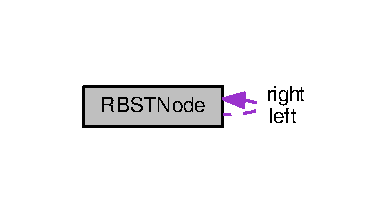
\includegraphics[width=187pt]{classRBSTNode__coll__graph}
\end{center}
\end{figure}
\subsection*{Public Member Functions}
\begin{DoxyCompactItemize}
\item 
\hyperlink{classRBSTNode_a2710c115f70614de3040b2c698e3a9cf}{R\+B\+S\+T\+Node} ()
\item 
\hyperlink{classRBSTNode_a2c0665d4b814a686ba8046d79204b8b3}{R\+B\+S\+T\+Node} (int ele)
\item 
\hyperlink{classRBSTNode_a96186cec6fe0f148c6f33090a9052783}{R\+B\+S\+T\+Node} (int ele, \hyperlink{classRBSTNode}{R\+B\+S\+T\+Node} $\ast$\hyperlink{classRBSTNode_aaed05c0dc1229e3ac9bfd48ca1f34c84}{left}, \hyperlink{classRBSTNode}{R\+B\+S\+T\+Node} $\ast$\hyperlink{classRBSTNode_a086e0e15cf51b06199e205eaeee17086}{right})
\end{DoxyCompactItemize}
\subsection*{Public Attributes}
\begin{DoxyCompactItemize}
\item 
\hyperlink{classRBSTNode}{R\+B\+S\+T\+Node} $\ast$ \hyperlink{classRBSTNode_aaed05c0dc1229e3ac9bfd48ca1f34c84}{left}
\item 
\hyperlink{classRBSTNode}{R\+B\+S\+T\+Node} $\ast$ \hyperlink{classRBSTNode_a086e0e15cf51b06199e205eaeee17086}{right}
\item 
int \hyperlink{classRBSTNode_a834716f43484069f09fb8fabf577b64e}{priority}
\item 
int \hyperlink{classRBSTNode_afe12defb7cc83803252973f1cd797464}{element}
\end{DoxyCompactItemize}


\subsection{Constructor \& Destructor Documentation}
\index{R\+B\+S\+T\+Node@{R\+B\+S\+T\+Node}!R\+B\+S\+T\+Node@{R\+B\+S\+T\+Node}}
\index{R\+B\+S\+T\+Node@{R\+B\+S\+T\+Node}!R\+B\+S\+T\+Node@{R\+B\+S\+T\+Node}}
\subsubsection[{\texorpdfstring{R\+B\+S\+T\+Node()}{RBSTNode()}}]{\setlength{\rightskip}{0pt plus 5cm}R\+B\+S\+T\+Node\+::\+R\+B\+S\+T\+Node (
\begin{DoxyParamCaption}
{}
\end{DoxyParamCaption}
)\hspace{0.3cm}{\ttfamily [inline]}}\hypertarget{classRBSTNode_a2710c115f70614de3040b2c698e3a9cf}{}\label{classRBSTNode_a2710c115f70614de3040b2c698e3a9cf}

\begin{DoxyCode}
23         \{
24             this->\hyperlink{classRBSTNode_afe12defb7cc83803252973f1cd797464}{element} = 0;
25             this->\hyperlink{classRBSTNode_aaed05c0dc1229e3ac9bfd48ca1f34c84}{left} = \textcolor{keyword}{this};
26             this->\hyperlink{classRBSTNode_a086e0e15cf51b06199e205eaeee17086}{right} = \textcolor{keyword}{this};
27             this->\hyperlink{classRBSTNode_a834716f43484069f09fb8fabf577b64e}{priority} = \hyperlink{RandomizedBinarySearch_8cpp_a4ce3e2af80a76d816ab7f8567ec4a65a}{MAX\_VALUE};         
28         \}    
\end{DoxyCode}
\index{R\+B\+S\+T\+Node@{R\+B\+S\+T\+Node}!R\+B\+S\+T\+Node@{R\+B\+S\+T\+Node}}
\index{R\+B\+S\+T\+Node@{R\+B\+S\+T\+Node}!R\+B\+S\+T\+Node@{R\+B\+S\+T\+Node}}
\subsubsection[{\texorpdfstring{R\+B\+S\+T\+Node(int ele)}{RBSTNode(int ele)}}]{\setlength{\rightskip}{0pt plus 5cm}R\+B\+S\+T\+Node\+::\+R\+B\+S\+T\+Node (
\begin{DoxyParamCaption}
\item[{int}]{ele}
\end{DoxyParamCaption}
)\hspace{0.3cm}{\ttfamily [inline]}}\hypertarget{classRBSTNode_a2c0665d4b814a686ba8046d79204b8b3}{}\label{classRBSTNode_a2c0665d4b814a686ba8046d79204b8b3}

\begin{DoxyCode}
31         \{
32             \hyperlink{classRBSTNode_a2710c115f70614de3040b2c698e3a9cf}{RBSTNode}(ele, NULL, NULL);         
33         \} 
\end{DoxyCode}
\index{R\+B\+S\+T\+Node@{R\+B\+S\+T\+Node}!R\+B\+S\+T\+Node@{R\+B\+S\+T\+Node}}
\index{R\+B\+S\+T\+Node@{R\+B\+S\+T\+Node}!R\+B\+S\+T\+Node@{R\+B\+S\+T\+Node}}
\subsubsection[{\texorpdfstring{R\+B\+S\+T\+Node(int ele, R\+B\+S\+T\+Node $\ast$left, R\+B\+S\+T\+Node $\ast$right)}{RBSTNode(int ele, RBSTNode *left, RBSTNode *right)}}]{\setlength{\rightskip}{0pt plus 5cm}R\+B\+S\+T\+Node\+::\+R\+B\+S\+T\+Node (
\begin{DoxyParamCaption}
\item[{int}]{ele, }
\item[{{\bf R\+B\+S\+T\+Node} $\ast$}]{left, }
\item[{{\bf R\+B\+S\+T\+Node} $\ast$}]{right}
\end{DoxyParamCaption}
)\hspace{0.3cm}{\ttfamily [inline]}}\hypertarget{classRBSTNode_a96186cec6fe0f148c6f33090a9052783}{}\label{classRBSTNode_a96186cec6fe0f148c6f33090a9052783}

\begin{DoxyCode}
36         \{
37             this->\hyperlink{classRBSTNode_afe12defb7cc83803252973f1cd797464}{element} = ele;
38             this->left = \hyperlink{classRBSTNode_aaed05c0dc1229e3ac9bfd48ca1f34c84}{left};
39             this->right = \hyperlink{classRBSTNode_a086e0e15cf51b06199e205eaeee17086}{right};
40             this->\hyperlink{classRBSTNode_a834716f43484069f09fb8fabf577b64e}{priority} = rand() % 100 + 1;
41         \}    
\end{DoxyCode}


\subsection{Member Data Documentation}
\index{R\+B\+S\+T\+Node@{R\+B\+S\+T\+Node}!element@{element}}
\index{element@{element}!R\+B\+S\+T\+Node@{R\+B\+S\+T\+Node}}
\subsubsection[{\texorpdfstring{element}{element}}]{\setlength{\rightskip}{0pt plus 5cm}int R\+B\+S\+T\+Node\+::element}\hypertarget{classRBSTNode_afe12defb7cc83803252973f1cd797464}{}\label{classRBSTNode_afe12defb7cc83803252973f1cd797464}
\index{R\+B\+S\+T\+Node@{R\+B\+S\+T\+Node}!left@{left}}
\index{left@{left}!R\+B\+S\+T\+Node@{R\+B\+S\+T\+Node}}
\subsubsection[{\texorpdfstring{left}{left}}]{\setlength{\rightskip}{0pt plus 5cm}{\bf R\+B\+S\+T\+Node}$\ast$ R\+B\+S\+T\+Node\+::left}\hypertarget{classRBSTNode_aaed05c0dc1229e3ac9bfd48ca1f34c84}{}\label{classRBSTNode_aaed05c0dc1229e3ac9bfd48ca1f34c84}
\index{R\+B\+S\+T\+Node@{R\+B\+S\+T\+Node}!priority@{priority}}
\index{priority@{priority}!R\+B\+S\+T\+Node@{R\+B\+S\+T\+Node}}
\subsubsection[{\texorpdfstring{priority}{priority}}]{\setlength{\rightskip}{0pt plus 5cm}int R\+B\+S\+T\+Node\+::priority}\hypertarget{classRBSTNode_a834716f43484069f09fb8fabf577b64e}{}\label{classRBSTNode_a834716f43484069f09fb8fabf577b64e}
\index{R\+B\+S\+T\+Node@{R\+B\+S\+T\+Node}!right@{right}}
\index{right@{right}!R\+B\+S\+T\+Node@{R\+B\+S\+T\+Node}}
\subsubsection[{\texorpdfstring{right}{right}}]{\setlength{\rightskip}{0pt plus 5cm}{\bf R\+B\+S\+T\+Node} $\ast$ R\+B\+S\+T\+Node\+::right}\hypertarget{classRBSTNode_a086e0e15cf51b06199e205eaeee17086}{}\label{classRBSTNode_a086e0e15cf51b06199e205eaeee17086}


The documentation for this class was generated from the following file\+:\begin{DoxyCompactItemize}
\item 
\hyperlink{RandomizedBinarySearch_8cpp}{Randomized\+Binary\+Search.\+cpp}\end{DoxyCompactItemize}

\chapter{File Documentation}
\hypertarget{RandomizedBinarySearch_8cpp}{}\section{Randomized\+Binary\+Search.\+cpp File Reference}
\label{RandomizedBinarySearch_8cpp}\index{Randomized\+Binary\+Search.\+cpp@{Randomized\+Binary\+Search.\+cpp}}
{\ttfamily \#include $<$iostream$>$}\\*
{\ttfamily \#include $<$cstdio$>$}\\*
{\ttfamily \#include $<$cstring$>$}\\*
{\ttfamily \#include $<$algorithm$>$}\\*
{\ttfamily \#include $<$cmath$>$}\\*
{\ttfamily \#include $<$vector$>$}\\*
{\ttfamily \#include $<$cstdlib$>$}\\*
Include dependency graph for Randomized\+Binary\+Search.\+cpp\+:
\nopagebreak
\begin{figure}[H]
\begin{center}
\leavevmode
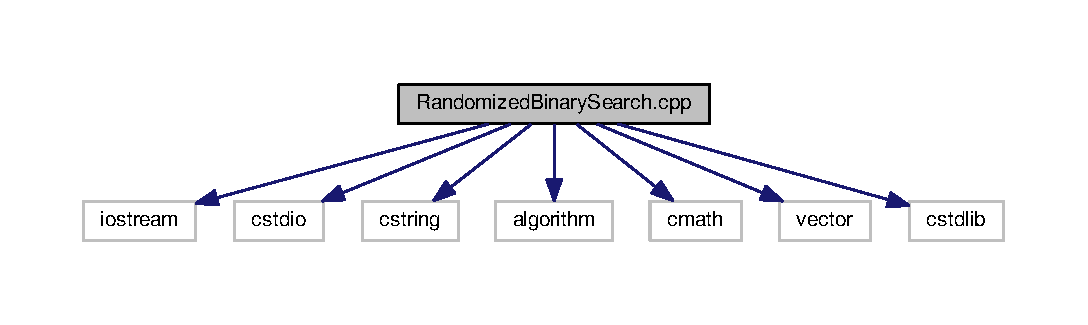
\includegraphics[width=350pt]{RandomizedBinarySearch_8cpp__incl}
\end{center}
\end{figure}
\subsection*{Classes}
\begin{DoxyCompactItemize}
\item 
class \hyperlink{classRBSTNode}{R\+B\+S\+T\+Node}
\item 
class \hyperlink{classRandomizedBinarySearchTree}{Randomized\+Binary\+Search\+Tree}
\end{DoxyCompactItemize}
\subsection*{Macros}
\begin{DoxyCompactItemize}
\item 
\#define \hyperlink{RandomizedBinarySearch_8cpp_a4ce3e2af80a76d816ab7f8567ec4a65a}{M\+A\+X\+\_\+\+V\+A\+L\+UE}~65536
\end{DoxyCompactItemize}
\subsection*{Functions}
\begin{DoxyCompactItemize}
\item 
int \hyperlink{RandomizedBinarySearch_8cpp_ae66f6b31b5ad750f1fe042a706a4e3d4}{main} ()
\end{DoxyCompactItemize}


\subsection{Macro Definition Documentation}
\index{Randomized\+Binary\+Search.\+cpp@{Randomized\+Binary\+Search.\+cpp}!M\+A\+X\+\_\+\+V\+A\+L\+UE@{M\+A\+X\+\_\+\+V\+A\+L\+UE}}
\index{M\+A\+X\+\_\+\+V\+A\+L\+UE@{M\+A\+X\+\_\+\+V\+A\+L\+UE}!Randomized\+Binary\+Search.\+cpp@{Randomized\+Binary\+Search.\+cpp}}
\subsubsection[{\texorpdfstring{M\+A\+X\+\_\+\+V\+A\+L\+UE}{MAX_VALUE}}]{\setlength{\rightskip}{0pt plus 5cm}\#define M\+A\+X\+\_\+\+V\+A\+L\+UE~65536}\hypertarget{RandomizedBinarySearch_8cpp_a4ce3e2af80a76d816ab7f8567ec4a65a}{}\label{RandomizedBinarySearch_8cpp_a4ce3e2af80a76d816ab7f8567ec4a65a}


\subsection{Function Documentation}
\index{Randomized\+Binary\+Search.\+cpp@{Randomized\+Binary\+Search.\+cpp}!main@{main}}
\index{main@{main}!Randomized\+Binary\+Search.\+cpp@{Randomized\+Binary\+Search.\+cpp}}
\subsubsection[{\texorpdfstring{main()}{main()}}]{\setlength{\rightskip}{0pt plus 5cm}int main (
\begin{DoxyParamCaption}
{}
\end{DoxyParamCaption}
)}\hypertarget{RandomizedBinarySearch_8cpp_ae66f6b31b5ad750f1fe042a706a4e3d4}{}\label{RandomizedBinarySearch_8cpp_ae66f6b31b5ad750f1fe042a706a4e3d4}
Display tree 
\begin{DoxyCode}
206 \{            
207     \hyperlink{classRandomizedBinarySearchTree}{RandomizedBinarySearchTree} rbst; 
208     cout<<\textcolor{stringliteral}{"Randomized Binary SearchTree Test\(\backslash\)n"};          
209     \textcolor{keywordtype}{char} ch;
210     \textcolor{keywordtype}{int} choice, item;
211     \textcolor{comment}{/*}
212 \textcolor{comment}{     * Perform tree operations  }
213 \textcolor{comment}{     */}
214     \textcolor{keywordflow}{do}    
215     \{
216         cout<<\textcolor{stringliteral}{"\(\backslash\)nRandomized Binary SearchTree Operations\(\backslash\)n"};
217         cout<<\textcolor{stringliteral}{"1. Insert "}<<endl;
218         cout<<\textcolor{stringliteral}{"2. Search "}<<endl;
219         cout<<\textcolor{stringliteral}{"3. Count Nodes "}<<endl;
220         cout<<\textcolor{stringliteral}{"4. Check Empty"}<<endl;
221         cout<<\textcolor{stringliteral}{"5. Clear"}<<endl;
222         cout<<\textcolor{stringliteral}{"Enter your choice: "};
223         cin>>choice;            
224         \textcolor{keywordflow}{switch} (choice)
225         \{
226         \textcolor{keywordflow}{case} 1: 
227             cout<<\textcolor{stringliteral}{"Enter integer element to insert: "};
228             cin>>item;
229             rbst.\hyperlink{classRandomizedBinarySearchTree_ae5d6d97456f3d4bca2b0f4b4e184dba3}{insert}(item);                     
230             \textcolor{keywordflow}{break};                          
231         \textcolor{keywordflow}{case} 2: 
232             cout<<\textcolor{stringliteral}{"Enter integer element to search: "};
233             cin>>item;
234             \textcolor{keywordflow}{if} (rbst.\hyperlink{classRandomizedBinarySearchTree_a3113d572e9cca081f0294fd47a994922}{search}(item))
235                 cout<<\textcolor{stringliteral}{"Element "}<<item<<\textcolor{stringliteral}{" found in the Tree"}<<endl;
236             \textcolor{keywordflow}{else}
237                 cout<<\textcolor{stringliteral}{"Element "}<<item<<\textcolor{stringliteral}{" not found in the Tree"}<<endl;
238             \textcolor{keywordflow}{break};                                          
239         \textcolor{keywordflow}{case} 3: 
240             cout<<\textcolor{stringliteral}{"Nodes = "}<<rbst.\hyperlink{classRandomizedBinarySearchTree_a6e7b0de6c0f6816b9785988e34c75dcb}{countNodes}()<<endl;
241             \textcolor{keywordflow}{break};     
242         \textcolor{keywordflow}{case} 4:
243             \textcolor{keywordflow}{if} (rbst.\hyperlink{classRandomizedBinarySearchTree_af35c367556914452ceba60569e95e5df}{isEmpty}()) 
244                 cout<<\textcolor{stringliteral}{"Tree is Empty"}<<endl;
245             \textcolor{keywordflow}{else}
246                 cout<<\textcolor{stringliteral}{"Tree is not Empty"}<<endl;
247             \textcolor{keywordflow}{break};
248         \textcolor{keywordflow}{case} 5: 
249             cout<<\textcolor{stringliteral}{"\(\backslash\)nRandomizedBinarySearchTree Cleared"}<<endl;
250             rbst.\hyperlink{classRandomizedBinarySearchTree_ae84229d93afdce90f4f0141a04c9736c}{makeEmpty}();
251             \textcolor{keywordflow}{break};            
252         \textcolor{keywordflow}{default}: 
253             cout<<\textcolor{stringliteral}{"Wrong Entry \(\backslash\)n "};
254             \textcolor{keywordflow}{break};   
255         \}
256  
258         cout<<\textcolor{stringliteral}{"\(\backslash\)nPost order : "};
259         rbst.\hyperlink{classRandomizedBinarySearchTree_aad0f82161d579cdb36990bbc72209be5}{postorder}();
260         cout<<\textcolor{stringliteral}{"\(\backslash\)nPre order : "};
261         rbst.\hyperlink{classRandomizedBinarySearchTree_a019f49873fd8e266eb41edc0af956b38}{preorder}();    
262         cout<<\textcolor{stringliteral}{"\(\backslash\)nIn order : "};
263         rbst.\hyperlink{classRandomizedBinarySearchTree_a2581cdb7ec61a153663a44a899f7d9ec}{inorder}();
264         cout<<\textcolor{stringliteral}{"\(\backslash\)nDo you want to continue (Type y or n) \(\backslash\)n"};
265         cin>>ch;                  
266     \} 
267     \textcolor{keywordflow}{while} (ch == \textcolor{charliteral}{'Y'}|| ch == \textcolor{charliteral}{'y'});               
268     \textcolor{keywordflow}{return} 0;
269 \}\end{DoxyCode}


Here is the call graph for this function\+:
\nopagebreak
\begin{figure}[H]
\begin{center}
\leavevmode
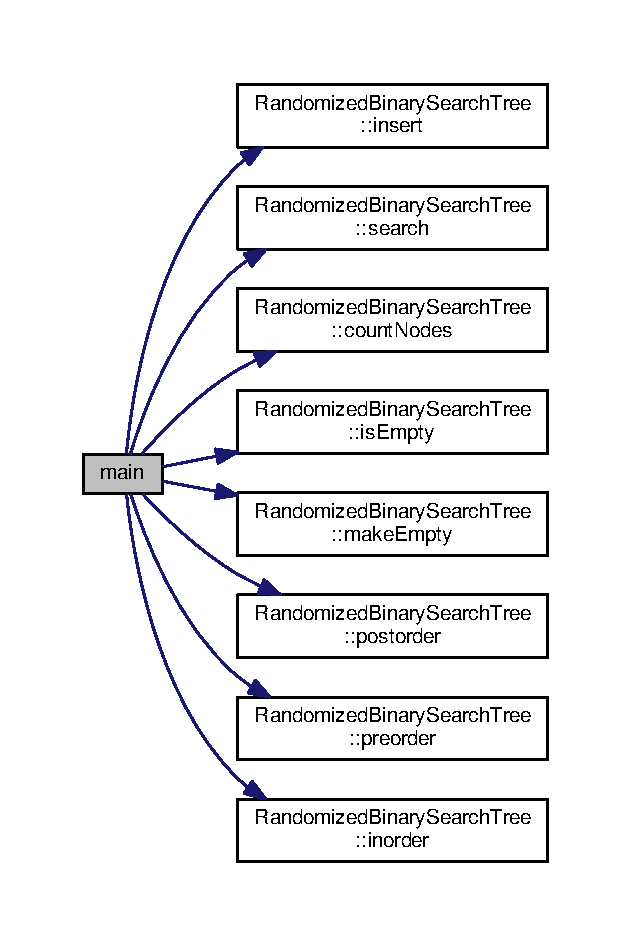
\includegraphics[width=303pt]{RandomizedBinarySearch_8cpp_ae66f6b31b5ad750f1fe042a706a4e3d4_cgraph}
\end{center}
\end{figure}



%--- End generated contents ---

% Index
\backmatter
\newpage
\phantomsection
\clearemptydoublepage
\addcontentsline{toc}{chapter}{Index}
\printindex

\end{document}
